\documentclass[preprint,12pt]{elsarticle} 

\vspace{5mm}



%=============================================================================
%\usepackage[margin=1.in]{geometry}
\usepackage{slashed}
\usepackage{graphicx}
\usepackage{amssymb}
\usepackage{mathtools}
\usepackage{bbold}
\usepackage{amssymb,latexsym}
\usepackage{amsmath,amsbsy,bbm}
\usepackage{multirow}
\usepackage[vcentermath]{youngtab}
\usepackage{nicefrac}
\usepackage[perpage]{footmisc}
\usepackage{wrapfig,lipsum,booktabs}
\usepackage{caption}
\usepackage{subcaption}
\usepackage{graphicx}
%\usepackage{physics}
\usepackage{floatrow}
\usepackage[dvipsnames]{xcolor} 
%\newfloatcommand{capbtabbox}{table}[][\FBwidth]
%=============================================================================
\newfloatcommand{capbtabbox}{table}[][0.45\textwidth]
\DefineFNsymbols*{lamportnostar}[math]{\dagger\ddagger\S\P\|{\dagger\dagger}{\ddagger\ddagger}}
\setfnsymbol{lamportnostar}
\renewcommand\thefootnote{\fnsymbol{footnote}}
%=============================================================================
\newcommand{\es}{1\text{\scriptsize s}}
\newcommand{\zs}{2\text{\scriptsize s}}
\newcommand*{\mprime}{^{\prime}\mkern-1.2mu}
\newcommand{\largescale}{\ensuremath{\Lambda_\text{Hi}}}
\newcommand{\lc}{\ensuremath{\Lambda_c}}
\newcommand{\fm}{\ensuremath{\,\text{fm}^{-1}}}
\newcommand{\abb}{\mbox{\ensuremath{A\oplus 1}}}
\newcommand{\red}[1]{\textcolor{red}{#1}} 
\newcommand{\green}[1]{\textcolor{green}{#1}} 
\newcommand{\blue}[1]{\textcolor{blue}{#1}} 
\newcommand{\lec}{C^\Lambda}
\newcommand{\led}{D^\Lambda}
\newcommand{\ddrei}[1]{\delta_{\tiny \Lambda}^{(3)}\!\big(#1\big)}
\newcommand{\wrt}{\textit{wrt.}~}
\newcommand{\etc}{\textit{etc.}~}
\newcommand{\eg}{\textit{e.g.}~}
\newcommand{\ie}{\textit{i.e.}~}
\newcommand{\eftnopi}{\mbox{EFT$(\not \! \pi)$}}
\newcommand{\ve}[1]{\ensuremath{\boldsymbol{#1}}}
\newcommand{\rms}[1]{\ensuremath{\langle r(#1)\rangle}}
\newcommand{\ls}{\ve{L}\cdot\ve{S}}
\newcommand{\be}{\begin{equation}}
\newcommand{\ee}{\end{equation}}
\newcommand{\bra}{\big\langle}
\newcommand{\ket}{\big\rangle}
\newcommand{\hl}{\big\vert}
\newcommand{\vcl}[1]{\ensuremath{\bar{\boldsymbol{r}}_\text{\tiny #1}}}
\newcommand{\vsp}[1]{\ensuremath{\boldsymbol{r}}_\text{\tiny #1}}
\newcommand{\la}{\label}
\newcommand{\figref}[1]{fig.~\ref{#1}}
\newcommand{\tabref}[1]{table~\ref{#1}}
%=============================================================================


\journal{PhysicsLetters B} 


\begin{document}
\begin{frontmatter}

\title{Multi-fermion systems with contact theories}
\author{M.~Sch{\"a}fer}
\address{Nuclear Physics Institute of the Czech Academy of Sciences, 25069 \v{R}e\v{z}, Czech Republic}
\address{Czech Technical University in Prague, Faculty of Nuclear Sciences and Physical Engineering, B\v{r}ehov\'{a} 7, 11519 Prague 1, Czech Republic}
\author{L.~Contessi} 
\address{Racah Institute of Physics, The Hebrew University, 91904 Jerusalem, 
Israel} 
\address{ESNT, IRFU, CEA, Universite Paris Saclay, F-91191 Gif-sur-Yvette, France} 
\author{J. Kirscher}
\address{Theoretical Physics Division, School of Physics and Astronomy,
The University of Manchester, Manchester, M13 9PL, United Kingdom} 
\date{October 2018}


\begin{abstract}
In this paper we numerically extend and study the effect of universality beyond totally spatially symmetric systems. 
No mixed angular momentum stable states can be found in the universal limit: in which the scattering length is much larger than the effective range.
This result has strong implications for any system close to universality, especially to nuclear physics, in which such stability is expected (e.g. $^6$He).
This points to the conclusion that momentumless contact theories can not qualitatively describe the nuclear chart and momentum dependent operators needs to be accounted to resolve the issue. 

We extend this study inspecting the role of the interaction range and studying this effect for different systems close to universality and realizations of discrete scale invariance.
\end{abstract}

\begin{keyword} 
P-wave systems, universality, contact effective field theory, unitarity, renormalization, pionless, stochastic variational method, resonating group method.
\end{keyword} 

\end{frontmatter}

%\newpage
%=============================================================================

\section{Introduction}

Quantum systems with a two-body scattering length much larger than the effective range $\frac{r_0}{a_0}\rightarrow 0$ are observed to follow similar behavior regardless of the energy scale of the problem or the inter-particle interaction detail.
These systems are therefore known as universal or scale invariant, and they can be found in the most disparate energy settings as hadronic, nuclear, and atomic physics ~(see, \eg,
Refs.~\cite{Tornqvist:1991ks,Voloshin:2003nt,Braaten:2003he,philli,tjon,PhysRevLett.81.69}).
One example of universal behaviour is the accumulation of infinite bound states at threshold in the three-bosonic system with a contact two-body interaction ($r_0\rightarrow0$) \cite{Efimov:1971zz}.
This also leads to the Thomas collapse \cite{PhysRev.47.903} and to the requirement of the inclusion of a three-body force to apply these theories to a physical and energetically-finite three-body configuration.
Doing so, the breaking scale invariance is broken (by the new three-body energy scale introduced) leaving only a weaker and discrete version of it.
In spite of that, many physical proprieties of few-body systems result to be merely consequence of universality and of the particular realization of the discrete scale invariance, which in return can be used to explain many physical behaviour in a very model-independent fashion.
Notable universal effects comprehend, the Tjon~\cite{tjon}~and Phillips~\cite{philli}~correlations, and the spectrum of the multi-boson system~\cite{manybosons}.
However, if consequence of universality in spatially totally symmetric systems are wildly studied [,,], very little is known for systems with higher internal angular momenta. 

Some information in this regard come from atomic and nuclear physics. 
O. I. Kartavtsev et al.  \cite{Kartavtsev_2007} showed that in the case of three two-component fermions, a contact theory ($r_0\rightarrow 0$) predicts a stable bound state only if the mass ratio between the two species is larger than $m_B/m_A \gtrapprox 13 $.
D. S. Petrov et al. \cite{petrov_dimerov, Petrov:2005zz,PhysRevA.92.053624} extended this result showing that if the fermions have the same mass, adding a fourth one the system does not bind as well.
Should be noticed that those two systems can not support Efimov effect as more than two fermions with two-internal-components can not be arranged in totally symmetric spatial wave functions.

In nuclear physics, the situation is more complex since the number of fermionic flavors is four and more particles can be arranged in a symmetric spatial wave function.
Within contact EFT framework, it was shown \cite{Contessi:2017rww} that $^{16}$O nucleus appears to be unstable with respect to four-$\alpha$ breaking.
Recently, Gattobigio et al. \cite{Gattobigio:2019omi} showed that also $^{6}$He is not stabilized by a momentumless short-range interaction with respect deuterium and $\alpha$ decay, but a stable bound state can be found if P-wave attraction is included nonperturbativly.
These two evidences point towards the possibility that theories with $a_0/r_0\rightarrow \infty$ are not able to stabilize systems with mixed spatial symmetry (in this paper referred as P-wave systems).
This effect can be a feature of universality, but it is certainly a disadvantage for physics that experimentally show this stability.
In this paper we analyze this issue using contact EFT (effective field theory) to approach the contact limit. 
At first we complement the studies done for few-nucleon systems that can be found in literature with 6-, 7-, and 8-body calculations.
Then we extend our description in what the authors think is the most promising scenario to find universal P-wave stable states.
In this respect, we look at O. I. Kartavtsev et al. work \cite{Kartavtsev_2007} in which the binding of two non-interacting identical fermions is induced by a third massive particle, when the mass ratio between the species is large enough.
For having a similar situation one can think of a system of $A+1$ particles, which includes a pair of identical fermions and $A-1$ particles forming a massive spatially symmetrical \textit{core} which might induce binding.
Increasing the number of particles in the core, the attraction with the extra fermions will be enhanced increasing the overall stability of the system.
Even if this scenario seems an artificial way of probing the configuration for the most probable binding, this situation can be found in atoms with large spin component (e.g. 9 spin-7/2 atoms [*which?*]) or in systems of two identical fermions in a bath of bosons with all the interactions similar and unitary (e.g. two polarized $^3$He atoms in a bath of zero temperature $^4$He).

However, as will be shown in this paper, we do not find evidences of P-wave binding even in this ideal scenario and changing the particular realization of three-body discrete scale invariance used.
Therefore, we conclude that the absence of P-wave stable states is a consequence of universality and is featured in all the systems at unitarity or with a contact S-wave interaction.
This absence has deep consequences for physics in several energy regimes but mostly in nuclear physics where such P-wave stability is expected, and for which realization, the relaxation of unitarity trough the inclusion of an additional scale might be required.



%=============================================================================
%\vspace{4mm}
\section*{Theory}
The minimal EFT for non-relativistic point particles exhibiting two- and three-body shallow states has been studied extensively (\eg~Refs.\cite{Lepage:1997cs,vanKolck:1999mw, Bedaque:1998kg, Braaten:2004rn, Hammer:2017tjm, Hammer:2019poc}).
The theory is defined as a perturbative series and can be refined systematically to attain a desired accuracy.
Its Hamiltonian formulation at leading order (LO) comprises zero-range two- and three-body vertices which depend on the renormalization parameter~$\Lambda$:

\begin{align}
H = - \sum_{i<j} \frac{\hbar^2}{2m}\ve{\nabla}_{ij}^2+ \lec \sum_{i<j}{\delta_\Lambda(\ve{r}_i-\ve{r}_j)} 
\,+\nonumber\\
\led \sum_{ i<j<k \atop \text{cyc} }\delta_\Lambda(\ve{r}_i-\ve{r}_j)\delta_\Lambda(\ve{r}_i-\ve{r}_k).
\label{eq:hamiltonian}
\end{align}

In the expansion of any resultant amplitude, the LO is represented by all Born
terms depending solely on the coupling constants $\lec$ and $\led$. 
Parameters representing the aforementioned refinements
enter perturbatively at the order given na\"ively by their mass
dimension. 
In this work, a Gaussian regulator 
\mbox{$\delta_\Lambda(\ve{x}) \propto\Lambda^3 e^{-\frac{\Lambda^2}{4}\ve{x}^2}$} is used.
The specific dependence of $\lec$ and $\led$ on $\Lambda$ thus induced, was calibrated to
the energy of a single state in the two- ($B(2)$) and three-body
($B(3)$) system, respectively.
Whether or not the $\Lambda$ convergence of another amplitude depends on the
specific choice for $B(2)$ and $B(3)$ classifies the corresponding observable as
universal or emergent.
The few-body problem is thereby specified at LO with four parameters: the particle's mass
(here, $m=938~$MeV), the number of particles and their statistics,
and the dimer and trimer binding energies.
The possibility of varying the cut-off and/or including sub-leading orders renders the contact EFT
a useful framework for studies of the universal regime.

We use this structure to consider both the nuclear scenario and a class of ($A+1$)-body equal-mass systems which contain only one pair of 
indistinguishable particles. Therefore, a subset of $A$ distinguishable particles obeys Bose statistics and can lay on a symmetrical
spatial wave functions, as stipulated in the introduction.
These arrangements will be referred to as \abb~as this notation has the advantage of immediately exposing the number of particle $A$ that, in a shell modern representation, can be arranged in a single shell (\eg , the $S$-shell).
We approach the unitarity limit in these systems by increasing the ratio \mbox{$\upsilon:=B(3)/B(2)$},
we assume exact unitarity with $B(2)=\epsilon$ in combination with $B(3)=3$~MeV, and a deviation from it with $B(2)=1$~MeV and $B(3)\in\lbrace3,\,4\rbrace$~MeV.
The nuclear case is renormalized to yield the deuterium and triton binding energies of $B(2)=2.22$~MeV and $B(3)=8.48$~MeV, respectively. 
We choose to drop any spin and isospin dependence of the interaction in accordance with the recent formulation~\cite{Konig:2016utl}
of $S$-shell nuclei in an expansion around the unitarity limit whose LO is (iso)spin symmetric.

The necessary fits for $\led$ employ Stochastic-Variational~(SVM,~\cite{Suzuki:1631377})~and
Resonating-Group~(RGM,~\cite{PhysRev.52.1083,hmh-rrgm})~variational diagonalizations. $\lec$ is
determined via a Numerov-type integration of the appropriate one-dimensional
radial Schr\"odinger equation.



%%%%%%%%%%%%%%%%%%%%%%%


%\hspace{2cm}
\section*{Results:}


\begin{figure}
\centering
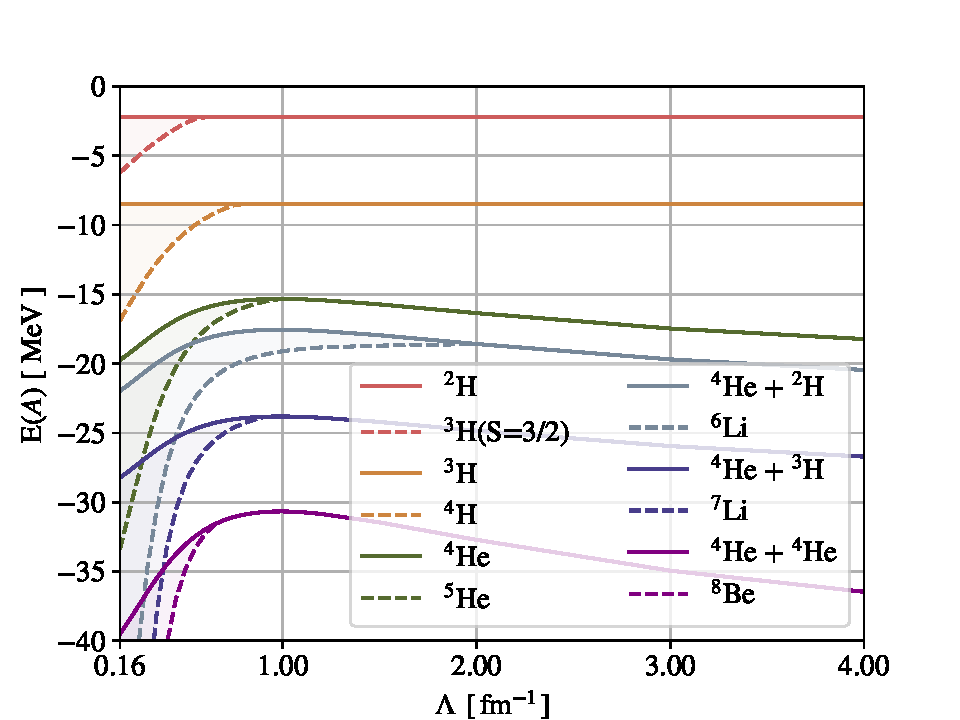
\includegraphics[width=\linewidth]{./Nuclear.pdf} 
\caption{Cutoff dependence of nuclear ground-state energies
obtained in LO~\eftnopi. For $A<5$, solid lines represent nuclei with
spatially symmetric ground-state wave functions. For $A>4$,
solid lines mark the lowest decay threshold into two spatially symmetric fragments.
The convergence of the energy with respect the cut-off was verified, up to $\Lambda\sim 10$fm$^{-1}$, to be in agreement with the expected $E\propto\tfrac{1}{\Lambda}$ behaviour \cite{Bedaque:1998kg, Barnea:2013uqa}, however, large cut-offs are omitted in the figure for sake of clarity.}
\label{fig:nuclear}
\end{figure}

Our results as obtained with the above defined theory
for the lowest energy eigenvalues of nuclear systems of up to eight nucleons are shown
in fig.~\ref{fig:nuclear},
where we find particle-stable $P$-wave nuclei (dashed lines) only below a critical cutoff $\lc<2\fm$.
For larger cutoffs, \ie, shorter-ranged interactions,
the unphysical quartet state of $^3$H is unstable \wrt~a decay into deuterium plus neutron, \mbox{$^4\text{H}\to\,^3\text{H} + n$},
\mbox{$^5\text{He}\to\alpha +n$}, \mbox{$^6\text{Li}\to\alpha+^2\text{H}$}, \mbox{$^7\text{Li}\to\alpha + ^3\text{H}$},
 and \mbox{$^8\text{Be}\to \alpha+\alpha$}.
The precise cutoff value below which a bound state exists is system dependent.
For systems with a decay channel into a single nucleon plus a composite, this critical range decreases as follows:
\mbox{$\lc(^3\text{H})<\lc(^4\text{H})<\lc(^5\text{He})$}. Whether this increase is driven by the decreasing spatial
 extend of the composite and/or
the number of distinguishable particles bound therein shall be discussed below (fig.~\ref{fig:RGM}).

Replacing the point-like nucleon with an $\alpha$ particle
in the decay channel -- note the implied increase in the number of nucleons with identical (iso)spin orientation -- the trend is opposite
for the positive-parity states: $\lc(^8\text{Be})<\lc(^6\text{Li})$.
Qualitatively, the exchange interaction between the decay fragments, which supports the nucleon-nucleon attraction,
can partially explain this hierarchy. The absence of an
effective angular momentum barrier further increases the attraction between the fragments. Apparently, the critical decrease
of interaction strength between certain pairs of nucleons (those with identical (iso)spin) in the zero-range limit, is reached
at shorter distances if the spatial extend of a fragment and its accompanying exchange interaction compensate.
It is beyond the scope of this work to quantify this observation, but the study below (fig.~\ref{fig:RGM}) is a first step
towards a deeper understanding of the interplay between the established EFT scales ($m_\pi$ and $\aleph$) and the statistical
properties which might in combination lead to additional low-energy scales. 

%
For the applicability of the pionless EFT to a nucleus the magnitude of $\lc$ when it decays from
bound to unbound matters. For all considered nuclei, we found this transition to occur at interaction ranges which are of the
same order or even smaller than the inverse nuclear breakdown scale (expected to be around the pion mass $m_\pi$).
The stability, \ie, the amplitude pole location on a fixed Riemann sheet, is therefore not invariant \wrt~appropriate RG transformations
($\Lambda\gg m_\pi$), \ie, in regions where the cutoff is expected to parametrize unobservable high-energy behaviour.
Hence, the three-parameter theory postdicts correctly only the experimentally established instability of nuclei in the
$^3\text{H}(\frac{3}{2}^-),\,^3n,\,^4\text{H},\,^{3,4}\text{Li},\,\text{and}~^5\text{He}$ channels.
The isotopes $^{6,7}\text{Li}$ and $^8$Be with $J^\pi=1^+$, $\frac{3}{2}^-$, and $0^+$, which are known to sustain stable
states\footnote{$^8$Be is considered to be stable without Coulomb repulsion~\cite{AFZAL:1969zz,Higa:2008dn}}
are not correctly reproduced in that aspect.
%
Interestingly, once a bound $^8$Be ground state is found with $J^\pi=0^+$ at $\Lambda<\lc$ the theory orders excited states in the
rotational spectrum correctly, namely, $0^+$, $2^+$, and $4^+$. 
The latter two states emerge in form of bound excited states for $\Lambda<0.4~{\rm fm^{-1}}$.

%
\begin{figure}
    \centering
        \centering
        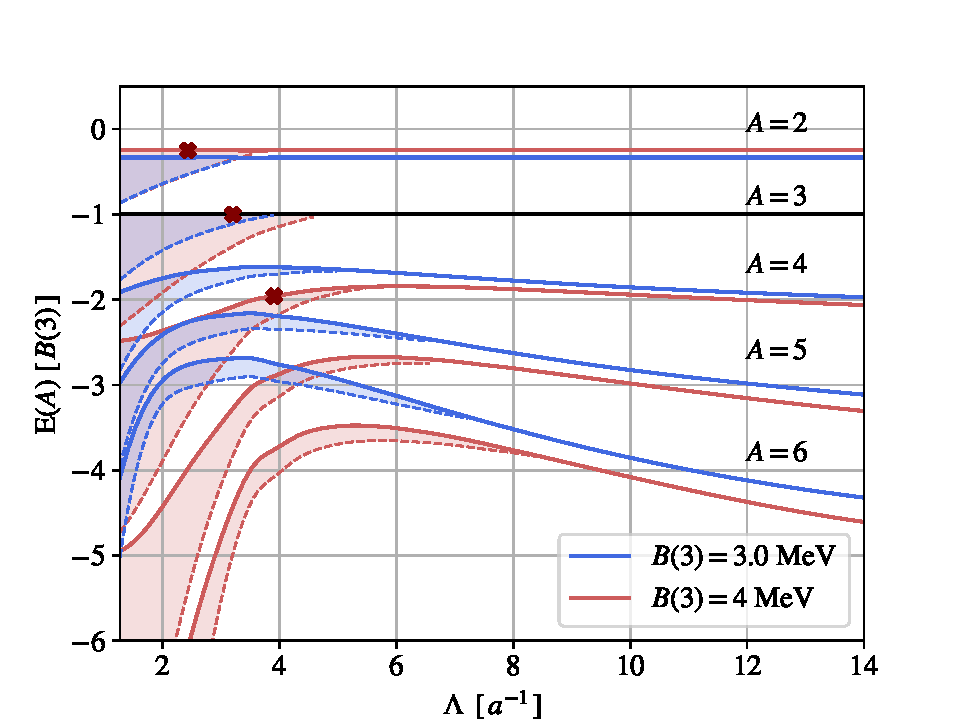
\includegraphics[width=\linewidth]{./p-systems-vs-l} 
        \caption{(LO Cutoff dependence of ground-state energies of $A$ spatially symmetric (solid) and \abb~mixed-symmetric systems
        (dashed) obtained with $B(2)=1~$MeV and $B(3)=3$ and $4~$MeV (blue and red) from equation \ref{eq:hamiltonian}. 
        The energies and the cut-off are represented in the natural scales, as function of $B(3)$ and scattering length $a_0$ respectively, this choice make possible the comparison of different $\upsilon$ but maks hard to represent the same quantity in the unitary limit with $a_0\rightarrow\infty$ and $\upsilon\rightarrow\infty$. 
        In the case of systems which can support total spatially symmetric groundstates, we find convergent behaviour as $\Lambda\to\infty$ (tested varying the cutoff between $1.2~a^{-1}<\Lambda<60~a^{-1}$) consistent with the one described in J.Carlson et al. study \cite{manybosons}.
        With scattering volume set to zero, the \abb~systems destabilize at smaller \lc~(red crosses, $B(3)=4$~MeV). 
        \red{change the graph to have $\upsilon$ in the key [and (maybe) we can express $\Lambda$ in B(3) as whell?] }}
        \label{fig:threshold}
\end{figure} 
%

Is this apparent inability of a contact EFT to stabilize a system of particles
which includes an undistinguishable pair dependent upon the fact that the nuclear interaction,
which we used above to exemplify this conjecture, realizes the unitarity condition only
approximately?
In order to assess the potential effect of the finite two-body scale (the deuteron),
we employed recalibrated EFTs (theory section) to obtain
at unitarity ($\upsilon\rightarrow \infty$) a ratio $B(4)/B(3)$ in agreement with 
Refs.~\cite{Hammer:2006ct,2009NatPh...5..417V}  as a benchmark.
In addition, \mbox{$B(A)/B(3)\Big\vert_{\upsilon=3}<B(A)/B(3)\Big\vert_{\upsilon=4}$}, implying that the universal ratios between the $A$- and 3-body energies is approached from below when taking the unitary limit.

Beyond distinguishable particles, we find systems with \abb~symmetry not stable in states with total orbital angular momentum $L_\text{total}=0$. This confirms the intuitive demand for mixed spatial symmetry due to the presence of an identical fermionic pair.
When projecting the spatial component of the wave function onto \mbox{$L_\text{total}=1$}, we find \abb~systems for $A$ between 2 and 6 to sustain stable states \mbox{($B(\abb)>B(A)$)} for small cutoffs (see fig.~\ref{fig:threshold} for $\upsilon<\infty$).
In approaching the contact limit by increasing the cutoff the \abb~systems become unbound at some critical value $\lc$.
%
This $\lc$ increases for an interaction which realizes the universal limit $\upsilon\rightarrow\infty$ more accurately 
and will thus support stable systems for a wider range of cutoffs (blue and the red lines in fig.~\ref{fig:threshold}).
For fixed $\upsilon$, $\lc$'s increase approximately linearly with the system size: \mbox{$\lc\propto A<7$}.
These observations suggest the existence of a finite $\lc$ close-to and at unitarity for arbitrarily large \abb~systems.
Hence, the stability of a given \abb~system is undetermined, even in the universal limit, and dependent upon the range of
the two-boson interaction, \ie, an additional scale.

\red{These two evidences seems to support the facts, which will be demonstrated to not be true, that the disintegration of such systems is an emerging effect and that increasing the number of particles might enforce stability.}

\begin{figure}
\centering
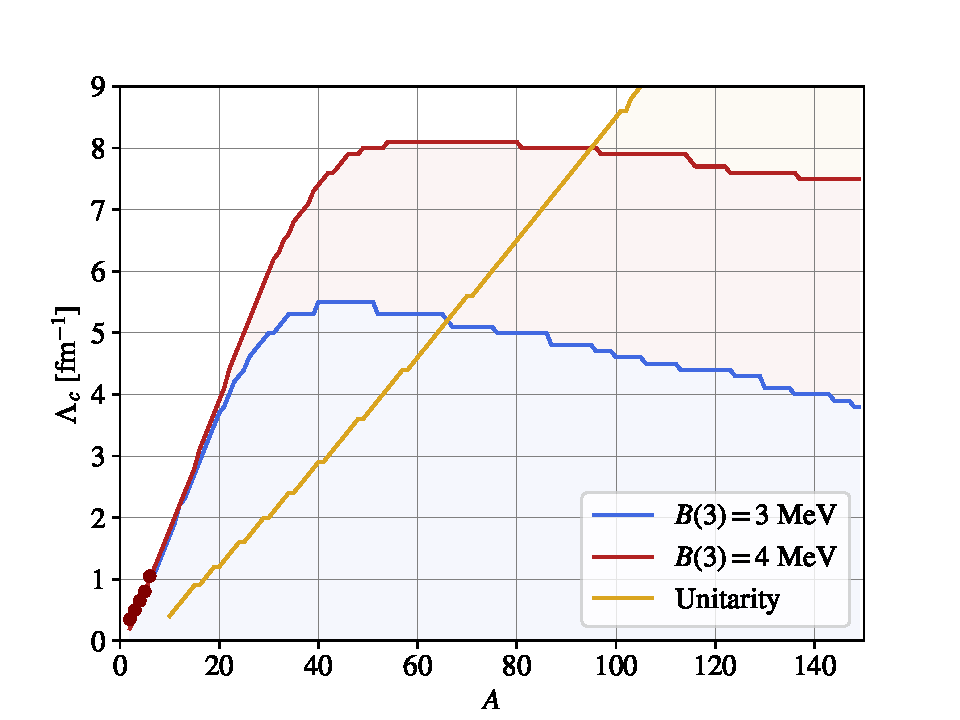
\includegraphics[width=\linewidth]{./RGM.pdf} 
\caption{Dependence of the critical cutoff $\lc$ on the number of core particles
$A$. SVM few-body results are shown for $A<7$ (dots, $B(3)=4~$MeV) along with single-channel resonating-group approximations for $A<150$ (lines). The unitarity limit
(yellow) was realized with $B(2)\to0^+$ and $B(3)=3~$MeV and deviations from it
with $B(2)=1~$MeV and $B(3)\in\lbrace3,4\rbrace~$MeV (blue, red). 
In the shaded regions, the respective theories do sustain bound \abb~states,
while systems above the lines are unstable.
The critical cut-off $\Lambda_c$ is expressed in fm$^{-1}$ (scale defined by the choice of the discrete scale symmetry breaking and the particle mass) to allow the rendering of the unitary limit as well, as each finite cut-off is to be considered extremely hard compared to the scattering length $a_0\rightarrow\infty$.
The step-like change in the curves results from a numerical criterion for the onset of binding and
can be removed systematically. 
\red{the key should be displayed in $\upsilon$ [and maybe the cut-off in b3?]}}
\label{fig:RGM}
\end{figure}


Results presented thus far, substantiate this hypothesis with results for $A>6$, only. To investigate conceivable deviations from
the linear dependence of $\lc$ on $A$, potential divergences in particular, we employ a two-fragment
local single-channel resonating-group approximation
(to be detailed in upcoming communication in extension of Refs.~\cite{PhysRev.52.1083,Naidon_2016}). 
This expansion formulates the (\abb)-body system as a two-body problem of a ``frozen'' core with $A$ particles and a residual
fermion which is forced out of their $S$-wave Pauli shell.
The halo character of the systems under consideration motivates a one-parameter representation of the symmetric core as a product of harmonic oscillator ground states, because the increasingly large gap between $B(A)$ and $B(A-1)$ does not allow for a core excitation
by the out-of-shell particle.
For $A<7$, this parameter is fitted to the SVM results for the rms radius of the core.
For larger $A$, we match the core wave function with the drop model formula $r_\text{rms}\propto A^{1/3}$ as 
it was found to be a good description for such systems in ref.~\cite{manybosons}.

Not at unitarity, we find $\lc(A)$ to abandon the linear increase found for small $A$.
$\lc$ increases up to a maximum number of particles $A^*$, while this maximum and the associated $\lc(A^*)$
both increase with $\upsilon$ (compare maxima of the blue and red curves in fig.~\ref{fig:RGM}). At unitarity,
we find a linear dependence recovered with any potential deviation to be found for $A>100$.
The existence of $A^*$ and the deviation from the linear $\Lambda_c\propto A$ relation thus appears to be an effect of deviating from unitarity.
In combination with the microscopic results, this confirms the main hypothesis of this work, namely that a system at unitarity cannot
support bound states in the zero-range limit if it contains indistinguishable particles.

Revisiting nuclear physics as a specific incarnation of this general class of systems,
its description with the \eftnopi~will not contain bound states with $A>4$.
In order to allow for the particle-stable character of $^{6,7}$Li and $^8$Be in the zero-range limit as a systematic
extension to LO \eftnopi, we analyse the mechanism behind the stability of these systems for $\Lambda<\lc$.
Of all artefacts introduced by the finite range of the regulated contact interaction,
a finite effective range in the two-body $S$-wave channel and a non-zero attractive two-body $P$-wave interaction are expected to dominate. 
Both contribute to the attraction in the \abb~system but their relative significance in this role is obscure.
In other words, the finite-range interaction does not only describe a large $S$-wave scattering length but
also other finite parameters of the effective-range expansion as the effective range $r_0$ and the scattering volume $a_1$.
To shed light on their relative importance, we project the two-body interaction into even partial waves.
An approximate $50\%$ reduction of $\lc$ for all $A$ is observed (purple crosses in \figref{fig:threshold})
as well as a decrease of equal proportion in the relative $P$-wave binding.
We infer from these results a similar significance of the finite $r_0$ and $a_1$ for the stability of the nuclear $P$-wave systems.
%

%
As in principle, theory must yield only the analytic structure of an amplitude in its range of validity,
without need to place the poles therein on the correct sheets, \ie,
RG-stable predictions for the character of a state are unnecessary as long as an RG-invariant pole
is predicted at all at LO which assumes its true bound, resonant, etc. character at higher orders. 
Above, we rules out bound-state poles without considering their fate once they intersect with threshold
at the critical cutoffs.
As a first step, we investigated the \abb~system with $A=2$.
This numerical study confirms the expectation
that at unitarity, a shallow $2\oplus1$ pole cannot be fixed to a specific energy.
In this limit, \ie, for a scale-invariant system, the resonance pole must not represent a scale and thus its location should either
merge with the threshold branch cut or diverge for $\Lambda\to\infty$\footnote{We thank U.~van~Kolck for clarifying discussions on this issue.}.
In the first case, three-body unitarity would be a universal consequence of the resonant two-body interaction. 
In the second case, the pole is an unphysical artefact which disappears with the regulator.
Our numerical results exhibit the latter behaviour. Specifically, the \abb~bound-state pole for $\Lambda<\lc$ hits threshold at $\lc$ and
moves away from this threshold for $\Lambda>\lc$.
However, for $A>2$, scale invariance is broken, and the associated emergence of a scale could in principle
pin the resonance to a finite energy. The pole trajectory for $A>2$ could thus be qualitatively different and
it remains to be calculated in order to advance the development of a contact EFT for $P$-wave systems.

%Such presence will tell whether a perturbative insertion of subleading order must move a shallow scattering pole to a stable one
%\footnote{At the present, the authors could not find any proof that the insertion of a perturbative interaction can (or can not)
% move a shallow T-matrix scattering pole into a stable one.}, or if a non-perturbative mechanism has to account for the creation
%  of the pole anew with the consequent revisiting of the theory LO.



%\vspace{4mm}
\section*{Conclusion}

We employ a 3-parameter non-relativistic contact EFT at LO for the description of $P$-wave nuclei with up to eight nucleons.
We find no bound states for these nuclei if the cutoff-renormalization scale of the theory exceeds a system-dependent critical value.
In addition to nucleons with their large but finite scattering length, we find systems which are arbitrarily close to unitary and realize
discrete scale invariance differently equally unstable for large enough cutoffs, \ie, in the zero-range limit.
This leads to the conclusion that systems whose dynamics is given by momentum-independent two- and three-body contacts, which are
constrained by spatially totally symmetric dimer and trimer states, are stable only if their spatial state is also totally symmetric.
States of mixed symmetry, as enforced by the presence of identical fermions in a system, are in turn predicted to be universally unstable. 

In order to generalize this result, and to assess the role of the ratio of distinguishable particles versus identical
particles in the system, we analyze $A$-body equal-mass systems with only one pair of identical particles within the EFT framework.
Thereby, we enforce a momentum-less contact interaction between all the particle pairs and triplets barring those which include the
identical pair. 
Also in this case which weakens the potential attraction due to the statistical properties in a minimal way, we find that these systems 
disintegrate in symmetrical spatial fragments -- a totally symmetric $A-1$-body core of distinguishable particles and one free particle
relative to it -- when the interaction cut-off is increased over a maximum value.
Both, number of particles (tested up to $A\sim150$) and proximity to the unitary limit stabilize the system for interactions of shorter range.
However, this range does not seem to converge to zero with either, implying that a pure contact theory is unable stabilize any mixed-symmetry
system. Having thus refuted the possibility of a combinatorial effect to conspire with the contact interactions to yield stable
mixed-symmetry states, momentum-dependent corrections left as the only means fit for this purpose.

\red{I think we should move this as too detailed into the results section}
%We stress that, a part of the ideal scenario in which the model do not contemplate the existence of further scales in the system, the application 
%of this theory to a physical system which would include a breaking scale $M$ given by high energy interaction components (\ie the existence of 
%meson exchanges in nuclear physics), would not change the conclusion of our analysis.
%In facts, as a finite $\lc$ indicates a drastic change of the system's behaviour, its magnitude being of the order of or even above (increasing 
%the number of particles) a conceivable breakdown scale would exclude this behaviour from the range of applicability of the theory.
%While, if $\lc\ll M$ the appearance of bound P-wave states should be interpreted as a cut-off artifact.

Therefore, for a future refined version of the above EFT which can be applied to systems with stable states of mixed symmetry,
nuclei in particular, we assess the effect of additional constraints on the theory: a finite two-body $S$-wave effective-range,
or a finite two-body $P$-wave scattering volume. 
Both were found of similar importance for the binding, and our study is thus inconclusive and cannot promote one parameter over the other.
Moreover, the way these corrections should be treated -- as a perturbation or in a non-perturbative fashion -- remains an open question.
While shallow, RG-stable poles might be stabilized with perturbative insertions of sub-leading operators, their absence demands for a
non-perturbative creation.
Whether or not such a mechanism which would pertain to any effective-field-theory formulation of systems close to universality,
which exhibit stability with mixed spatial symmetry as nuclei do most prominently, has to be implemented follows logically from
this work as a next stage. The answer will eventually allow for a universal understanding of seemingly different fields, where as of now,
Bose-like atoms and $S$-shell nuclei could be paralleled. 

\paragraph*{Acknowledgments}
We thank N.~Barnea,  M.~Birse, U.~van Kolck, J.~Mare\v{s}, N.~Walet for insightful
discussions.
M.S. was supported by the Czech Science Foundation GACR Grant No.19-19640S.
L.C. and J.K. acknowledge support from ``Espace de Structure et de r\'eactions
Nucl\'eaire Th\'eorique''  (ESNT, http://esnt.cea.fr )  at CEA-Saclay, where this work
was partially carried out.
L.C. was also supported by the Pazy Foundation and by the
Israel Science Foundation Grant No. 1308/16.

%=============================================================================



\bibliographystyle{ieeetr}
\bibliography{Thebibliography.bib}
\end{document}